

\documentclass[letterpaper, 10 pt, conference]{IEEEtran}  % Comment this line out
                                                          % if you need 
\usepackage{graphicx}
\usepackage{algorithm}% http://ctan.org/pkg/algorithm
\usepackage{algpseudocode}% http://ctan.org/pkg/algorithmicx
\usepackage{textcomp}
\usepackage{amssymb}
\usepackage{authblk}
\usepackage{caption}
\usepackage{subcaption}
\usepackage{subfig}
\usepackage{float}


\title{\LARGE \bf
Analysing Interesting Patterns in Large Multivariate Time Series Data using Shapelet
}

\author{R.N. Navagamuwa}
\author{K.J.P.G. Perera}
\author{M.R.M.J. Sally}
\author{L.A.V.N. Prashan}
\author{H.M.N. Dilum Bandara}
\affil[1]{Department of Computer Science and Engineering\protect\\ University Of Moratuwa\protect\\ Katubedda, Sri Lanka \authorcr Email: {\tt (randika.12, jaward.12, pravinda.12, prashan.12, dilumb)@cse.mrt.ac.lk} \vspace{-2ex}} 

\begin{document}
\graphicspath{ {images/} }


\maketitle
\thispagestyle{empty}
\pagestyle{empty}


%%%%%%%%%%%%%%%%%%%%%%%%%%%%%%%%%%%%%%%%%%%%%%%%%%%%%%%%%%%%%%%%%%%%%%%%%%%%%%%%
\begin{abstract}

Analyzing interesting patterns in large multivariate time series data have marked its own importance in allowing users to obtain useful insights of the stored data. Existing techniques are both computationally expensive and require extensive human interaction. In addressing these issues, we propose a technique that combines both parallel coordinates and shapelets. First each time instance of the multivariate time series is represented as a line on a set of parallel coordinates. Then a shapelet learning algorithm is applied to those lines on the parallel coordinates. Finally, identified shapelets are ranked based on their information gain.  This technique is computationally and memory efficient, and also enables users to focus only the shapelets with relevant information gains (high or low depending on the application) which is optimized using the shapelet extraction technique.  We demonstrate the utility of the proposed technique using a set of real-world datasets. 

\end{abstract}

\begin{IEEEkeywords} 
Parallel Coordinates;  Shapelets; Multivariate Time Series; Pattern Analysis 
\end{IEEEkeywords}

%%%%%%%%%%%%%%%%%%%%%%%%%%%%%%%%%%%%%%%%%%%%%%%%%%%%%%%%%%%%%%%%%%%%%%%%%%%%%%%%
\section{INTRODUCTION}

Analyzing interesting patterns in large, multivariate time series datasets are useful in many application domains [1]. For example, Complex Event Processing (CEP) [3] combines data from multiple, streaming sources to identify meaningful events or patterns in real time. These event may be as simple as reaching a predefined threshold and patterns could be as complex as a state diagram. While detection of relevant events and patterns may give insight about opportunities and threats related to the data being monitored (e.g., set of sensor readings and credit card transactions), ability to write CEP queries to detect such events and patterns require a significant domain knowledge. Manual analysis of data streams is not only tedious and error prone, but also important events are likely to be missed due to the limited domain knowledge of the query writer. A promising alternative is to automating the CEP query generation by automatically extracting/mining interesting patterns from the past data [3], [4], [5].

Time series pattern mining and classification techniques are extensively studied in literature. Dynamic Time Warping (DTW) [11] is one such technique used to measure the similarity between two time series based on a distance measure. However, the computational complexity of DTW grows exponentially with large and multiple time series limiting its usages. Furthermore, the accuracy of the results depends on the chosen sliding window, which is nontrivial to estimate [3]. Shapelets [1] is a set of time series classification technique that can be applied to any time series. A shapelet is a subsequence of a time series that is identified as being representative of class membership. While shapelets are fast, it only applies to a single time series. Ultra-fast shapelets [3] are proposed for multivariate time series analysis. Ultra-fast shapelets calculates a vectorized representation of respective attributes of the dataset. Then a  random forest is trained to identify the shapelets with respect to the total dataset. Leafs of the random forest are considered to be the symbols. The number of occurrences of a symbol in the raw data is counted and these symbol histograms are used for the final classification step using random forests. One of the main limitations of ultra-fast shapelets is the inefficiency in providing interpretations using the obtained shapelets regarding the analysis of identified patterns to the general users [8]. This occurs when learning shapelets for multivariate time series using random forests. Moving on ultra-shapelet implementation also fails to identify data columns dynamically into the shapelets. 
Furthermore majority of the developed systems has its own limitations in focusing only on specific domain related datasets. We argue on this issue as the system functionalities restricts only to specific domain which would reduce the usability of the system itself in large [10].

We propose a technique that represents the given multivariate time series data as a set of parallel coordinates and extract shapelets out of those coordinates to identify the interesting patterns. We argue interesting patterns as  anomalies, commonalities as well as time series breakpoints of a given dataset. Furthermore our approach dynamically chooses data columns (parallel coordinates) into respective shapelets. The percentage of the calculated information gain on the shapelets assist in deriving interpretation as the analysis on the identified patterns. 

Section 2 explains the related work with respect to the focused research area. Section 3 in the paper introduces to the problem statement, along with an illustrated example. Section 4 describes the proposed approach and section 5 contains a detailed explanation on the general architecture. Section 6 explains the performance analysis with respect to our approach. Concluding remarks and future work are explained in section 7.


\section{RELATED WORK}

This area being a highly research intensive are there had been major past work carried out in various related aspects targeting the focused domain. Following explanation describes directly related past work with respective to the focused domain.

\subsection{Shapelets}

Shapelets can be used for classification of time series, and Shapelets can be defined as time series subsequences which are in some sense maximally representative of a class. We can convert a dataset into two dimensional representation of time series, and that representation can be used for classification [1].  

\begin{figure}
\centering
\parbox{9cm}{
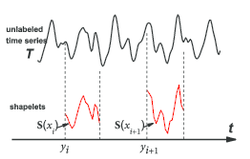
\includegraphics[width=9cm]{shapelet1.png}
\caption{Sationhapelets Represent}
\label{fig:2figsA}}
\qquad
\begin{minipage}{9cm}
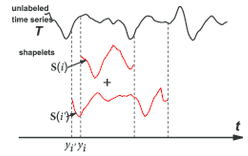
\includegraphics[width=9cm]{shapelet2.png}
\caption{Different length of Shapelets}
\label{fig:2figsB}
\end{minipage}
\end{figure}

In shapelets, classification will be done based on the shapes of data with time series. Many subsections can be created in a shape as in Fig. 1, and those subsections are called Shapelets. Fig. 2 represents different set of shapelets which can be extracted from a data stream.

\subsection{Parallel coordinates}

The parallel coordinates technique is widely used for the analysis of multivariate data [6].Parallel coordinates is a way of representing multidimensional data so that we can analyze them. For n dimensional space,  there are n parallel lines in a parallel coordinate system. Parallel coordinates can be drawn for a dataset consist of multiple columns. Thus there are multiple parallel lines (or axes for each column) are defined. When scaling these coordinate systems, defining a standard to represent data accurately is better than representing raw data unless data set would be biased to certain dimensions. So we can simply take the Standard normal distribution values for each columns and then represent data in the coordinate system. Fig. 3 shows an example Parallel Coordinate System.
\begin{figure}[h!]
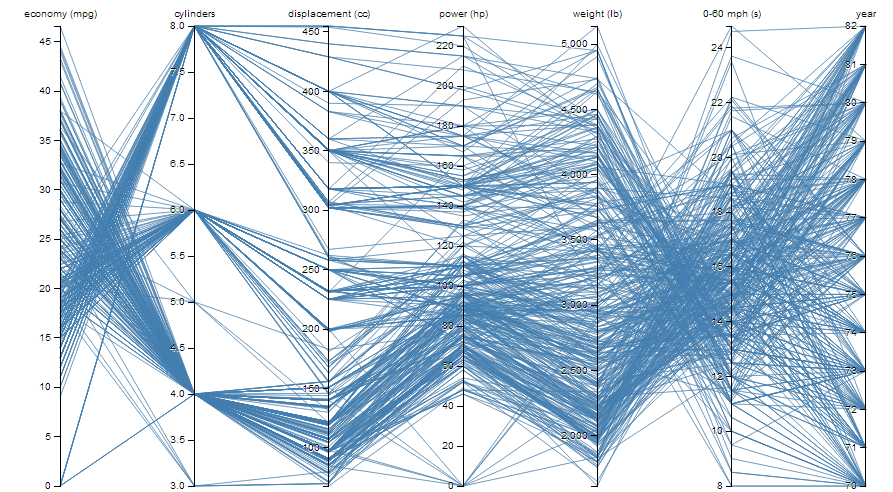
\includegraphics[width=0.5\textwidth]{parrelel.png}
\caption{Parallel Coordinate Representation}
\end{figure}

\subsection{Univariate and multivariate time series}

A time series is simply a time dependent function. For instance, velocity-time graphs and Acceleration-time graphs can be taken. Thus a univariate time series is a function of one variable which is dependent on time whereas Multivariate time series is a set of functions where each function is a representation of an attribute (a column) of the dataset. All the attributes values are depended on one time axis in this Multivariate Time Series [7].
 

\subsection{Problem Statement} 
The problem of pattern recognition in multivariate time series involves learning patterns in multivariate time series domain. We address the problem of automatic pattern recognition and analysis in large multivariate time series domain. Several related work have been carried out in trying to automate the process of identifying interesting patterns. However, they rely on strict assumptions such as dataset is an univariate time series and end user will be a domain expert [3][9].

In this paper to conduct our research using shapelets in parallel coordinates we used “Air Quality” dataset provided in UCI Machine Learning Repository [12]. This is a multivariate time series dataset which has 15 attributes. The dataset contains real world data.

The obtained dataset is converted into parallel coordinates from which the shapelets are identified. Each identified shapelet contains information regarding to which row the shapelet is identified, its length and the parallel coordinates (respective data columns) used in constructing the shapelet. Most importantly in order to construct more accurate shapelets we did transform the parallel coordinates (data points) using the standard normalization into a single comparable region. These shapelets represents the identified interesting patterns.  

Next would be the analysis and the interpretation of the identified patterns. In order to complete the analysis, calculation of the information gain of the identified shapelets would be required. In order to optimize the information gain calculation procedure the class label classification of the dataset is required. Simply in order to fulfill that requirement if the dataset is not classified we would cluster the given dataset in order to identify class labels relevant to each row. The Air quality sensor dataset was classified using three attributes Temperature (T), Relative Humidity (RH), Absolute Humidity (AH). 

In conducting the analysis, the obtained percentage values of the information gain calculation and the percentage values of the dataset classification will be mapped against each other comparing it values. The unmapped shapelets will be the outlier patterns and the mapped shapelets will contain the parallel coordinates (data points) relevant to the interesting events. In this use case we managed to extract 462 shapelets from the given dataset (“Air Quality”).  Fig. 4 shows all the extracted shapelets after sorting according to the information gain.
\begin{figure}[h!]
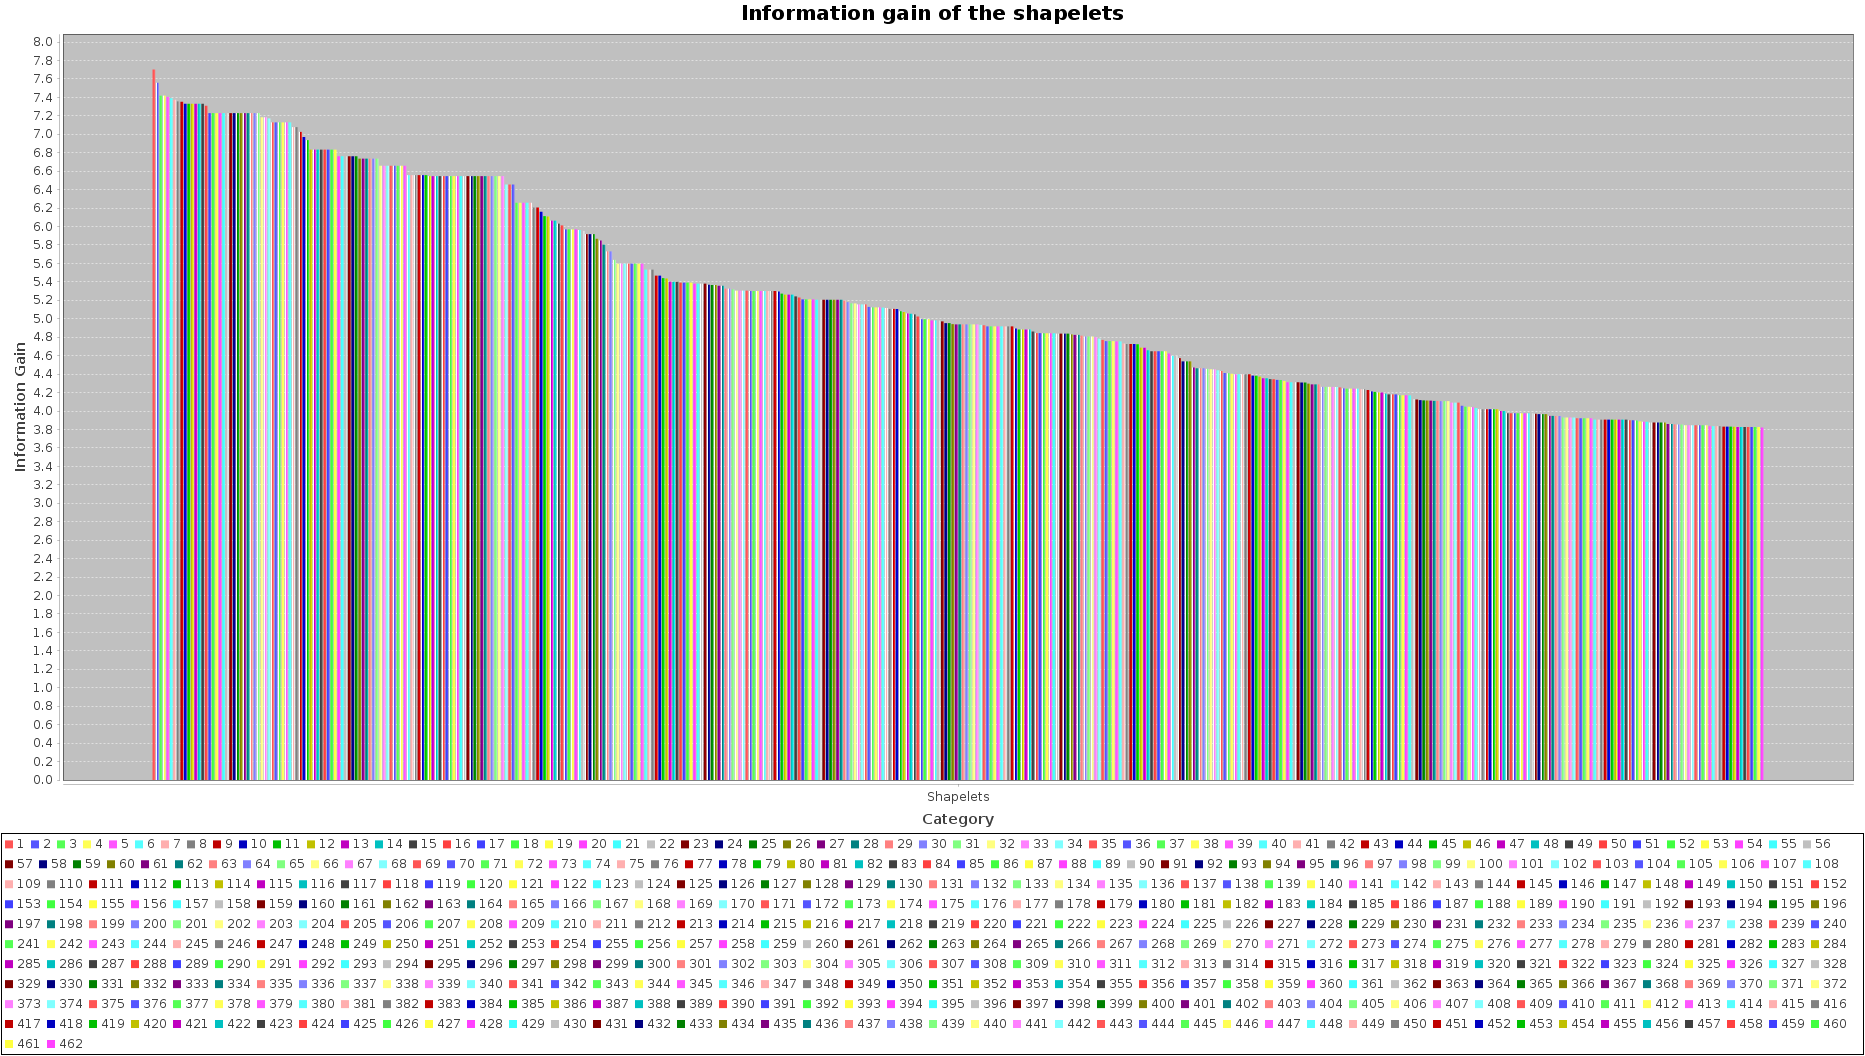
\includegraphics[width=0.5\textwidth]{shapeletGraph.png}
\caption{Information gain of the extracted shapelets}
\end{figure}


\subsection{The Proposed Approach}
Our proposed approach will have two separate phases which is described in Fig. 6

\begin{itemize}
\item Extract all possible shapelets from a given data set.
\item Identify important shapelets from the generated shapelets.
\end{itemize}

Few and recent efforts that touched about Shapelets are discussed in [1][2][3]. In this paper we introduce a new approach to define Shapelets using parallel coordinates as a vector of four dimensions s=(g,i,a,c), where g is the information gain which represents how much similar the data set for the shapelet, i is the series id which represents the row id of the data set, a is the starting column id and c is the content of data. Before extracting shapelets from the given dataset, the dataset will be transformed into a parallel coordinates system. In the proposed solution we transform the obtained dataset into  parallel coordinates in order to extract shapelets. The given fig-x displays an image of the obtained parallel coordinates (Only Temperature, Relative Humidity and Absolute Humidity considered) and these coordinates will be used to extract shapelets. Furthermore the Fig. 6 clearly segregates two classes within the dataset. The calculation of the percentage of the information gain will then be used to analyse the identified patterns against the obtained events within the system.
\begin{figure}[h!]
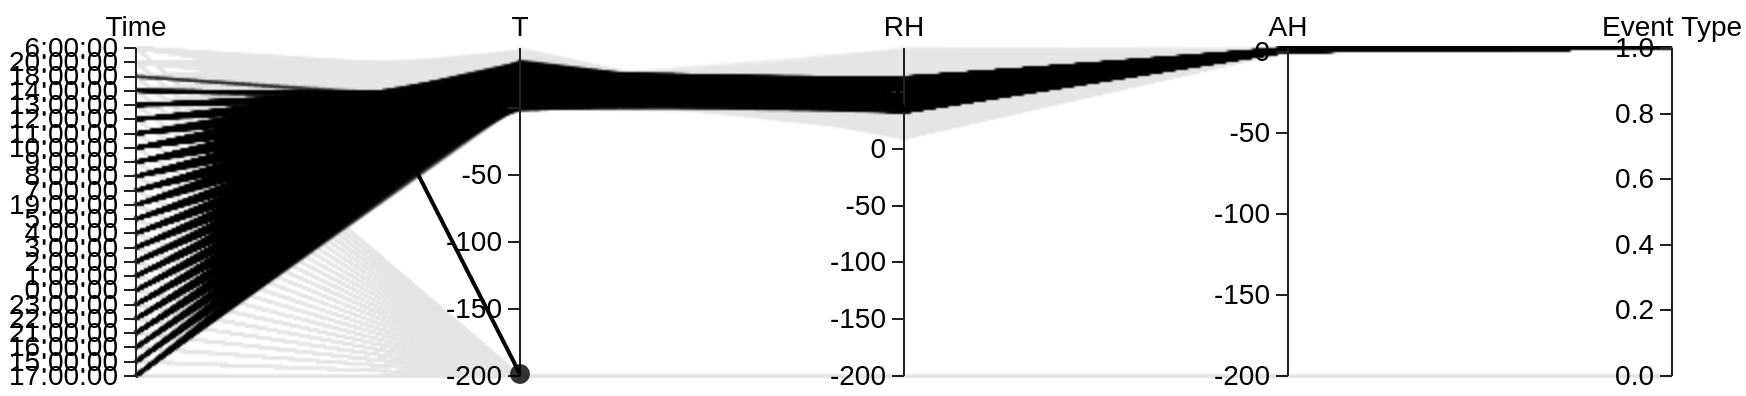
\includegraphics[width=0.5\textwidth]{airQuality.png}
\caption{Representation of parallel coordinates for Air Quality dataset(Only 4 columns are taken into consideration}
\end{figure}

Though the information gain is not used in this phase, it is defined in this phase. It will be used in the next phase. With respect to the length of the shapelets we could decide the minimum and maximum length of the Shapelet.  In this approach we take each and every row into the account and extract shapelets from every row as much as possible. If we take a row containing n number of columns and tries to extract shapelets from that row, maximum and the minimum lengths of the shapelets should be given to the system. Then the system tries to extract maximum possible shapelets from the dataset.

Learned shapelets are now taken for the second phase. Here the solution derives the best shapelets which would become the representatives of each of the classes or the classified parts of the dataset out of all the constructed shapelets. The algorithm is a process of comparing probability values of shapelets and the dataset. Comparing shapelets will be done based on the information gain. First it categorise each shapelet according to its probability (or proportion) of class value and then it is put to the relevant set. Then in each  set of shapelets, we calculate the minimum difference between each shapelets probability and the whole set’s probability. Finally the process derives the best matching shapelet for each category.

\section{General Architecture}
Our method builds upon two main phases which is described in Fig. 5.
\begin{figure}[h!]
\includegraphics[width=0.5\textwidth]{Architecture.png}
\caption{General Architecture of the system}
\end{figure}

\subsection{Phase one: Shapelet Learner}
Shapelets Learning phase encapsulates the logic for generating the the shapelets.
\begin{itemize}
\item Inputs : A dataset should be given as one of the inputs. As the second input Maximum and the Minimum lengths of the shapelets should be given. Default minimum length will be two and maximum length will be the column count.
\item Outputs : All the generated shapelets are the output of the first phase.
\end{itemize}
In this phase we developed our own algorithm to learn shapelets. Shapelets will be generated using Algorithm 1.

\begin{algorithm}[H]
  \caption{Shapelet Learner Algorithm}\label{shapeletLearner}
  \begin{algorithmic}[1]
    \Procedure{ShapeletLearner}{$D,MaxLength,MinLength$}\Comment{Time series dataset D and shapelet length}
     \State $shapelets \gets \{\}$
      \For{\texttt{each row r in D}}
      	\State $wholeCandidate \gets r$
        \State \texttt{length = MinLength}
        \While{\texttt{length <= MaxLength}}
        \State \texttt{length ++}
        \State \texttt{start = 0}
        	\While{\texttt{start <= r.length}}
            \State \texttt{start ++}
            \State $candidate \gets \{\}$
            \State \texttt{m = start}
            	\While{\texttt{m<start + length}}
                	\State \texttt{m++}
                    \State $\texttt{candidate[m-start]}\gets \texttt{wholeCandidate[m]}$
                \EndWhile
                \State $\texttt{finalCandidate} \gets \textbf{zNorm(}\texttt{candidate}\textbf{)}$
                \State \texttt{shapelets.add(finalCandidate)}
            \EndWhile
        \EndWhile
      \EndFor
      \State \textbf{return} $shapelets$\Comment{generated shapelets will e returned}
    \EndProcedure
  \end{algorithmic}
\end{algorithm}



All possible shapelets will be extracted from a given dataset. In addition to the Algorithm 1 the dataset will be standardized in to a normal distribution and based on that shapelets will be extracted. Extracted shapelets can be saved into a database or simply use as the input for the second phase. 

\subsection{Phase two : Shapelet Extraction}
Generated shapelets can be used as the input for this phase.
\begin{itemize}
\item Inputs : Generated shapelets and class values
\item Outputs : Important shapelets
\end{itemize}

Each generated shapelet contains a double array as the content. As the first step in the second phase we try merging shapelets and reduce the shapelet count. Information gain will be used to sort the extracted shapelets. Using Algorithm 2, number of extracted shapelets will be reduced. 

\begin{algorithm}[H]
  \caption{Shapelet Merger Algorithm}\label{shapeletMerger}
  \begin{algorithmic}[1]
     \Procedure{ShapeletMerger}{$S,Size$}\Comment{Shapelet Array S sorted according to information gains and size of the cluster}
     \State $shapelets \gets \{\}$
     \State $mergedShapelet \gets \{\}$
      \State $maxInfo \gets \textbf{findMaximumInfoGain(} \texttt{shapelets} \textbf{)}$
      \State $minInfo \gets \textbf{findMinimumInfoGain(} \texttt{shapelets} \textbf{)}$
      \State $thresholdVal \gets \texttt{(maxInfo - minInfo)/size}$
      \State $mergedShapelet \gets \texttt{0}$
      \State \texttt{mergedShapelet.add(shapelet[i])}
      \State \texttt{i++}
      \While{\texttt{minInfo<maxInfo}}
      \If{\textbf{size(}\texttt{S[i]}\textbf{}}
      \State \texttt{mergedShapelet.add(S[i])}
      \State \texttt{i++}
      \EndIf
      	\If{\texttt{minInfo >}\textbf{infoGain(}\texttt{S[i]}\texttt{)}}
        \State \texttt{minInfo += threshold}
        \State \texttt{shapelets.add(mergedShapelet)}
        \State $mergedShapelet \gets \texttt{0}$
       \State \texttt{mergedShapelet.add(shapelet[i])}
        \EndIf
      \EndWhile
      \State \textbf{return} $shapelets$\Comment{generated shapelets will be returned}
    \EndProcedure
  \end{algorithmic}
\end{algorithm}


We define a new shapelet, which contains several different shapelets. Since the newly generated shapelet contains more than one shapelet, it has a two dimensional double array as the content. These generated shapelets (With two dimensional double array as the content) will be used as the input for our next algorithm,Shapelet Finder Algorithm.  


\begin{algorithm}[H]
  \caption{Important Shapelet Finder Algorithm}\label{shapeletFInder}
  \begin{algorithmic}[1]
     \Procedure{GetImportantShapelets}{$S,classValues,data$}
     \State $\texttt{shapeletArr} \gets \{\}$
     \State $\texttt{classValueProb} \gets \{\}$
     \For{\texttt{classValue c in classValues}}
     \State $\texttt{shapeletBucket(c)} \gets \{\}$
     \State $\texttt{classValueProb.add(}  \textbf{findProbs(}\texttt{data,c))}$
     \EndFor
     \For{\texttt{each shapelet in S}}
     \State $\texttt{classVal} \gets \textbf{maxProbClassVal(} \texttt{shapelet} \textbf{)}$
     \State \texttt{shapeletBucket(classVal).}\textbf{put(}\texttt{shapelet}\textbf{)}
     \EndFor
     \State $\texttt{differences} \gets \{\} \{\}$
     \State $\texttt{minDifferences} \gets \{\}$
     \For{\texttt{classValue c in classValues}}
     \For{\texttt{shapelet in shapeletBucket}}
     	\State $\texttt{differences[c][shapelet.id]} \gets \textbf{}{abs(} \texttt{shapelet.prob - classValueProb[c])}$
     \EndFor
     \State $\texttt{minDifferences[c]} \gets \textbf{getMinDif(}\texttt{differences(c))}$
     $\texttt{newShapelet} \gets \textbf{getMinimumDiffShapelets(}
     \texttt{minDifferences[c],c}\textbf{}$
     \State \texttt{shapeletArr[c].add(newShapelet)}
     \EndFor
      \State \textbf{return} $shapeletArr$\Comment{generated shapelets will be returned}
    \EndProcedure
  \end{algorithmic}
\end{algorithm}

Procedure takes three parameters, Merged Shapelets, Class Values, Class Valued Dataset. Line 2 and 3 initilise two arrays named \textit{shapletArr}  and \textit{classValueProb}. Then for each class value a SET data structure is created named \textit{shapeletBucket}. And for each class value the probability of each class value is added to the \textit{classValueProb} array. \textbf{findProb()} funtion calculate the probability (proportion) of the relevant class value from the dataset. In the next step, each shaplet is put into a relevent \textit{shapletBucket}.

 \textbf{maxProbClassVal()} is a function that finds the maximum probability of being relevant class value of the shapelet.  Next the algorithm finds the absolute differences of the probabilities of the category and each shaplet within that category. Then for each category, it calculates the Minimum difference by \textbf{getMinDif()} function and then the relevant shapelet by \textbf{getMinimumDiffShaplets()} . All the derived the shaplets are added to the \textit{shapeletArr} and it’s returned. 

Note : Here the class value is an integer representation for each categories classified for the Dataset.

\section{Performance Analysis}
This section presents a detailed performance evaluation of analysing patterns in multivariate time series using shapelets. From our experimental results, we claimed that shapelets can be used to detect patterns in a large multivariate dataset without an domain expert inputs to the system. For the process we have taken 9358 instances from Air Quality dataset, and it was subjected to generate shapelets using our proposed approach. This experimental results claims that shapelets are more efficient compared in terms of time complexity as well as in detecting anomalies, commonalities as well as time series breakpoints without human interaction.  

Rare itemset pattern mining (AprioriRare) [13] technique is not suitable for detecting frequently occurring rare items, since it ignores high frequent events, but our approach can specifically identify all rare items using the obtained information gain. During our experiments, one of the key factors that we identified was the ability to optimize the information gain calculation procedure by providing the dataset classification into the shapelet information. If the provided dataset is a classified dataset then we would not have the burden of classifying it explicitly, but if not the classification using a clustering technique will allow us to figure out the cluster identity which the each row would belong to, and figuring out that will allow us to embed that information to the respective shapelets and optimize the information gain calculation. 

 
As the dataset grows larger the number of generated shapelets also increases in large. In dealing with large number of shapelets the accuracy goes down rapidly and as a solution for that we used a shapelet merging technique to merge similar shapelets based on a threshold difference stated upon the information gain. Furthermore as the dataset grows larger the previously previous research works related to DTW technique becomes inefficient. DTW uses a sliding window in order to compute the necessary distances, and in doing so as the dataset gets larger the accuracy gets lower as we need to define a sliding window of a better size which covers the total data distribution. The output accuracy directly depends on the decided window size.
Furthermore in obtaining parallel coordinates (data points) into the shapelets we transformed all the parallel coordinate values using standard normalization in order to make each and every data field comparable.


\section{CONCLUSION \& FUTURE WORK}

Shapelets are subsequences of functions or curves. Proposed solution identifies shapelets in the whole dataset and store relevant attributes for each shapletes. Information gain, Starting position and Shapelets contents are important attributes for further processes. First phase of the solution does this shapelets learning process using shapelet learning algorithm. Second phase is related with the classified values of the dataset where it finds a relationship with shapelets and the classified dataset. It happens by comparing informations gains and probabilities of occurrences of shapletes.  

As extended future work the current implementation would be extended to generate queries which would be processed through a complex event processor (CEP Engine). The data points (parallel coordinates) which would be necessary to build up the query is already identified within the shapelet. So the future work would be a continuation of the current work which we have described in this paper. Successful conclusion of this will allow us to totally automate the process of query generation for complex event processing. 

Furthermore, there is a considerable amount of future work with respect to optimizing the classification of a non-classified dataset, the information gain calculation procedure, shapelet learner and shapelet extraction techniques. 
 

\begin{thebibliography}{99}

\bibitem{c1} L. Ye and E. Keogh, "Time series shapelets," pp. 947–956, Jun. 2009. [Online]. Available: http://dl.acm.org/citation.cfm?id=1557122. Accessed: Aug. 7, 2016.
\bibitem{c2} O. Patri, A. Sharma, H. Chen, G. Jiang, A. Panangadan, and V. Prasanna. Extracting discriminative shapelets from heterogeneous sensor data. In Big Data, 2014 IEEE International Conference on. IEEE, 2014.
\bibitem{c3} R. Mousheimish, Y. Taher, and K. Zeitouni, "Complex event processing for the non-expert with autoCEP," pp. 340–343, Jun. 2016. [Online]. Available: http://dl.acm.org/citation.cfm?id=2933296. Accessed: Jul. 24, 2016.
\bibitem{c4} A. Margara, G. Cugola, and G. Tamburrelli. Towards automated rule learning for complex event processing. Technical report, Technical Report, 2013.
\bibitem{c5} A. Margara, G. Cugola, and G. Tamburrelli, "Learning from the past," pp. 47–58, May 2014. [Online]. Available: http://dl.acm.org/citation.cfm?id=2611289. Accessed: Jul. 24, 2016.
\bibitem{c6} J. Johansson and C. Forsell, "Evaluation of parallel coordinates: Overview, Categorization and guidelines for future research," IEEE Trans. Visual. Comput. Graphics, vol. 22, no. 1, pp. 579–588, 2016.
\bibitem{c7} X. Liu, S. Swift, A. Tucker, G. Cheng, and G. Loizou, "Modelling Multivariate time series,". 
\bibitem{c8} Wistuba, M., Grabocka, J. and Schmidt-Thieme, L. (2015a) Title: Ultra-fast Shapelets for time series classification. Available at: http://arxiv.org/abs/1503.05018
\bibitem{c9} H. Obweger, J. Schiefer, M. Suntinger, P. Kepplinger, and S. Rozsnyai, "User-oriented rule management for event-based applications," pp. 39–48, Nov. 2011. 
\bibitem{c10} Kavelar, A., Obweger, H., Schiefer, J., Suntinger, M.: Web-Based Decision Making for Complex Event Processing Systems. In: 6th World Congress on Services, pp. 453–458 (July 2010)
\bibitem{c11} Ratanamahatana, C. and Keogh, E. 2004a. Everything you know about dynamic time warping is wrong. In Proceedings of the 3rd Workshop on Mining Temporal and Sequential Data. 1--11.
\bibitem{c12} "UCI machine learning repository: Air quality data set," 2016. [Online]. Available: http://archive.ics.uci.edu/ml/datasets/Air+Quality.
\bibitem{c13} L. Szathmary, A. Napoli, and P. Valtchev, "Towards rare Itemset mining," 19th IEEE International Conference on Tools with Artificial Intelligence(ICTAI 2007), 2007. [Online]. Available: http://www.philippe-fournier-viger.com/spmf/apriorirare.pdf. Accessed: Aug. 8, 2016.


\end{thebibliography}




\end{document}
